\documentclass[11pt]{article}

\usepackage[a4paper,margin=1.8cm]{geometry}
\emergencystretch=1em
\usepackage{graphicx}
\usepackage{array}
\usepackage{booktabs}
\usepackage{amsmath}
\usepackage{amssymb}
\usepackage{float}
\usepackage{subcaption}
\usepackage[hidelinks]{hyperref}
\usepackage{xurl}
\usepackage{caption}
\usepackage{enumitem}
\captionsetup{font=small,labelfont=bf}
\graphicspath{{../MT2026012/figures/}}

\usepackage{xcolor}
\usepackage{titlesec}
\usepackage{fancyhdr}
\definecolor{accent}{HTML}{8A5A2B}
\definecolor{sectionblue}{HTML}{1F4E5F}
\titleformat{\section}{\normalfont\Large\bfseries\color{sectionblue}}{\thesection}{0.6em}{}
\titleformat{\subsection}{\normalfont\large\bfseries\color{accent}}{\thesubsection}{0.6em}{}
\titleformat{\subsubsection}{\normalfont\normalsize\bfseries\color{accent}}{\thesubsubsection}{0.6em}{}
\titlespacing*{\section}{0pt}{3ex plus 0.5ex minus 0.3ex}{0.7ex plus 0.1ex}
\titlespacing*{\subsection}{0pt}{2.4ex plus 0.4ex minus 0.2ex}{0.5ex plus 0.1ex}
\titlespacing*{\subsubsection}{0pt}{1.9ex plus 0.3ex minus 0.2ex}{0.4ex}

% --- title block spacing (reduced, still larger than section gaps) -------
\makeatletter
\renewcommand\@maketitle{%
  \newpage
  \null
  \vskip 1.2em%
  \begin{center}%
    {\LARGE \@title \par}%
  \end{center}%
  \par
  \vskip 2em}
\makeatother
\setlength{\headheight}{14pt}
\pagestyle{fancy}
\fancyhf{}
\fancyhead[C]{\color{accent}\rule{\textwidth}{0.8pt}}
\renewcommand{\headrulewidth}{0pt}
\renewcommand{\footrulewidth}{0.8pt}
\renewcommand{\footrule}{\color{accent}\hrule height 0.8pt}
\fancyfoot[C]{\thepage}

\title{\textbf{Machine Learning Course Project-I}\\[0.3em]
       \large Flight Price Prediction (Regression)}
\date{}

\begin{document}
\maketitle

\section*{Team Name: Carrot}
\begin{center}
\small
\begin{tabular}{@{}>{\raggedright\arraybackslash}p{3.4cm}l>{\raggedright\arraybackslash}p{9.2cm}@{}}
\toprule
Name & Roll number & Contribution \\
\midrule
Aradhya Chakrabarti & MT2026012 & Preprocessing for the flight competition (data loading, cleaning and feature engineering); Models Tested: linear regression (OLS), polynomial regression, Ridge, Lasso, decision trees, random forests (with cross-validation, evaluation and hyperparameter tuning) \\
Ankit Lamba & MT2026122 & Exploratory testing and data analysis for the flight competition; tested SVR, linear regression and random forest baselines \\
Kunal Yadav & MT2026047 & Ran preliminary prediction experiments for the flight competition \\
Kshitij Beri & MT2026046 & Implemented an ensemble model (blend) of trees, forests and boosting; achieved the team's best public leaderboard score on the flight competition \\
\bottomrule
\end{tabular}
\end{center}

\section*{Source code}
The full code for this competition is in the project repository: \url{https://github.com/TimeATronics/AIT511_Project1}

\section{Problem and dataset}

We are given a regression problem: predict the ticket price (in USD) of a US domestic flight. The training file \texttt{train.csv} has 18,076 rows and 12 columns, and the test file has 4,520 rows and 11 columns. The columns are airline, flight, source\_city, destination\_city, departure\_time, arrival\_time, stops, flight\_class, duration (hours), days\_left, and the target price. The evaluation metric is $R^2$.

We have used the following models: linear regression (ordinary least squares), polynomial regression, Ridge (L2), Lasso (L1), decision trees, and random forests, along with various experimentations and combinations of the same.

\section{Data loading}

We begin by loading the three CSV files (training, test and the sample submission) with pandas. Both files turn out to be complete: there are no duplicate rows and no missing cells in either file, so no imputation is needed in practice. We still keep a median/mode imputer inside the pipeline so that the code would not break if missing values appeared later.

\section{Exploratory data analysis}
\subsection{Data distribution check (skewness)}

For EDA, the first thing we check is the shape of the target, since it decides which error metric is sensible and whether a transformation could help the linear models. We compute the descriptive statistics along with skewness and kurtosis, and plot the raw prices next to $\log(1+\text{price})$ (Figure~\ref{fig:flightdist}).


From the histogram we see that most tickets are concentrated below USD 400, while a handful of fares reach USD 8,996 against a median of only USD 234. The computed skewness (7.07) and kurtosis (170.25) quantify how strongly these few expensive tickets pull the distribution away from the typical fare. Since the models are scored with squared error, these few tickets can dominate the score.

\begin{figure}[H]
\centering
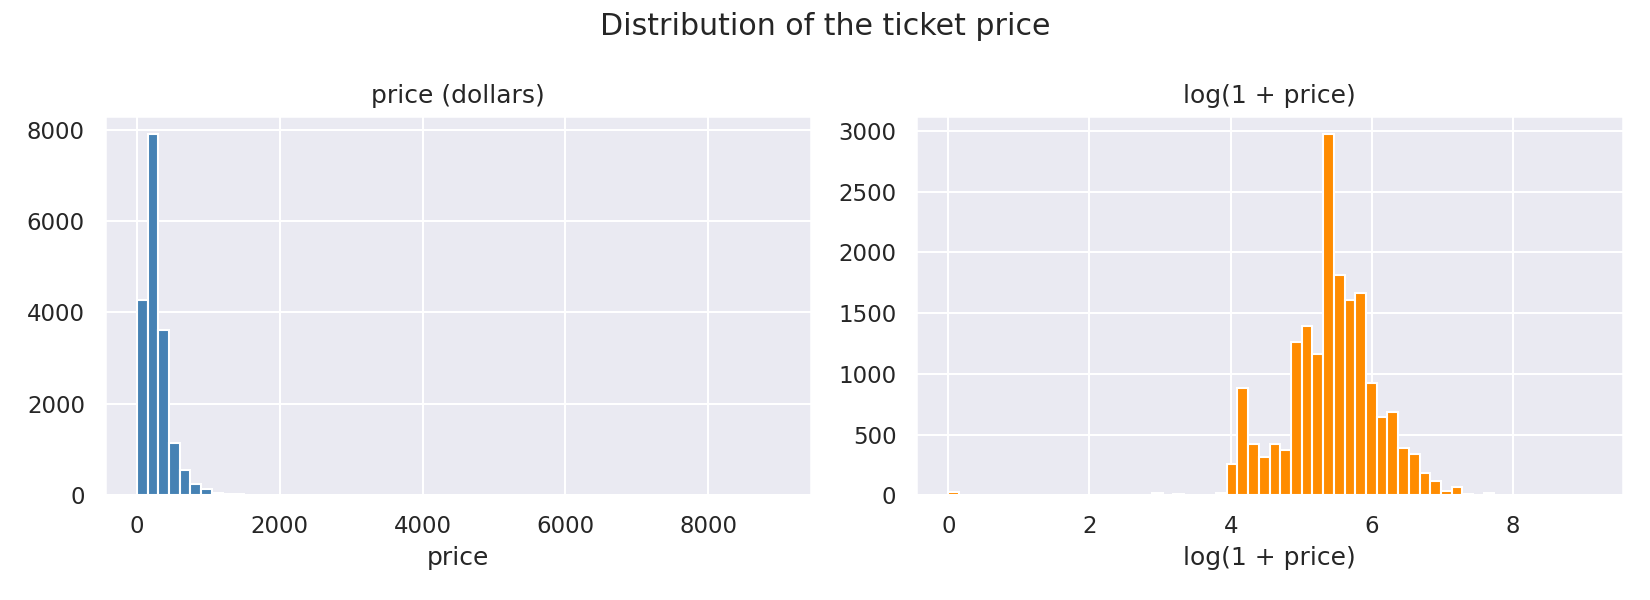
\includegraphics[width=0.78\linewidth]{flight_price_distribution.png}
\caption{Price distribution in raw dollars and after $\log(1+\text{price})$.}
\label{fig:flightdist}
\end{figure}

\subsection{Feature-wise analysis}

Next we look at the two numeric features and at how price behaves across the categorical ones. The code prints the descriptive statistics of \texttt{duration} and \texttt{days\_left}, their correlations with price, and draws boxplots for the numeric columns and for price across seating class, stops and airline (Figure~\ref{fig:flightcat}). Accordingly, we observe the following:

\begin{itemize}
  \item Business tickets are clearly higher in price, with median near USD 320 against USD 194 for Economy. Business class has the outlier expensive fares near USD 8,996.
  \item Non-stop flights have a median near USD 214, while one-stop and two-or-more itineraries are around USD 347 and USD 370. Only 193 flights have two or more stops, so that group is relatively small.
  \item Airline medians range from about USD 168 for Frontier up to about USD 260 for United, Delta and Alaska. Southern Airways Express appears exactly once in the training data, so nothing general can be learned for it.
  \item \texttt{duration} ranges from 0.87 to 28.65 hours, though a few flights run much longer than the rest, and \texttt{days\_left} covers 1 to 44 days. Neither relates strongly to price since the linear correlations are only $+0.281$ and $-0.229$.
\end{itemize}

\begin{figure}[H]
\centering
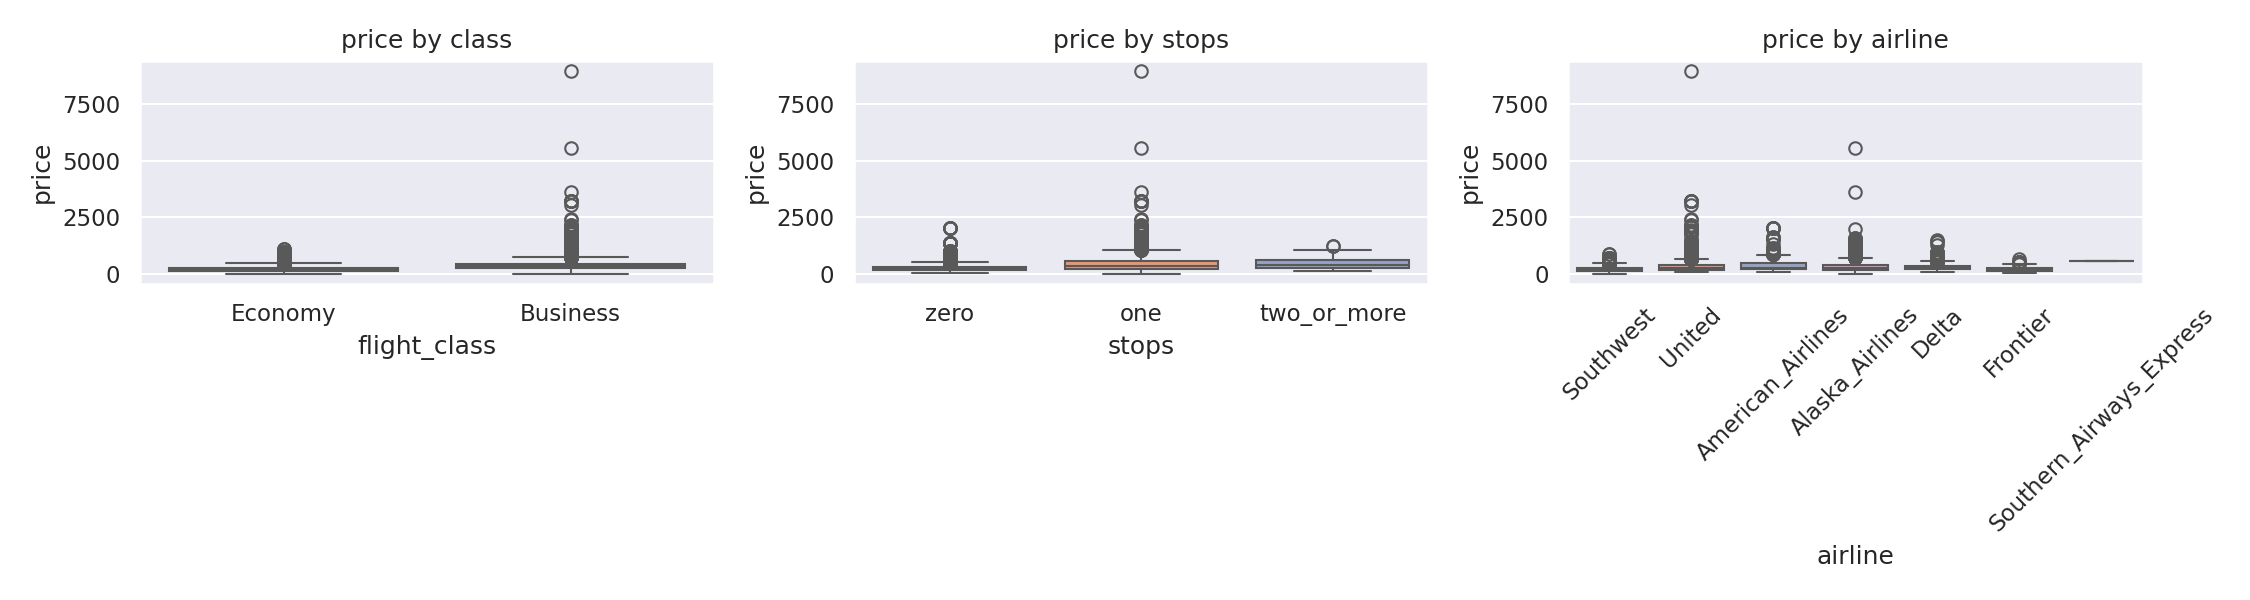
\includegraphics[width=\linewidth]{flight_price_by_category.png}
\caption{Price by seating class, number of stops and airline.}
\label{fig:flightcat}
\end{figure}

\subsection{Correlation analysis}

We then check the correlations between the numeric columns. The heatmap block shows that no pair is strongly linearly related, and the largest correlation with price is $+0.28$ for \texttt{duration}. A linear model trained only on the numeric columns would probably perform not as well as models considering the categorical columns as well. See Section~\ref{sec:families}.

\subsection{High-cardinality columns}

Finally, we inspect the categorical cardinalities. \texttt{flight} has 1,123 distinct codes, and 33 of them appear only in the test file. Treating it as a category would create over a thousand sparse columns and the unseen codes would have no coefficients at all, so we replace it with engineered features in Section~\ref{sec:features}.

\section{Data cleaning}

For cleaning, we find 25 training rows with a price of 0. Since a ticket cannot cost nothing, these look like entry errors and we remove them; 18,051 rows remain for training. 

\section{Feature engineering}\label{sec:features}

We build three features from existing columns:

\begin{enumerate}
  \item \texttt{airline\_code} and \texttt{flight\_number} from the flight code. For example, the code ``WN 3596'' contains the carrier (``WN'') and a serial number, and airlines tend to reuse numbers for the same route, so the number can carry route information that the city columns would not convey.
  \item \texttt{stops\_ordinal}: \texttt{stops} is one-hot encoded during preprocessing for the regression models.
  \item \texttt{route}: source and destination are merged into one category. The same city pair have the same fare level this way.
\end{enumerate}

\section{Data preprocessing}

All preprocessing is done with a scikit-learn \texttt{ColumnTransformer} and used inside a \texttt{Pipeline}, so during cross-validation (CV) every transformation is fitted on the training folds only and the not the validation folds.

\begin{itemize}
  \item Numeric columns are imputed with the column median and standardised for the models that need it. Scaling is done for the regression models with penalization (Ridge and Lasso). Trees split on thresholds and use raw values.
  \item Categorical columns are imputed with the most frequent value and one-hot encoded, with the \texttt{handle\_unknown} option set to \texttt{"ignore"}.
  \item Columns with more than 100 levels are dropped by the encoder; \texttt{flight} is the only such column.
\end{itemize}

\section{Model evaluation}

For targets $y_i$ and predictions $\hat{y}_i = f(x_i;w)$, we report
\[
  \mathrm{MSE} = \frac{1}{n}\sum_{i=1}^{n}(y_i-\hat{y}_i)^2, \qquad
  \mathrm{RMSE} = \sqrt{\mathrm{MSE}}, \qquad
  \mathrm{MAE} = \frac{1}{n}\sum_{i=1}^{n}|y_i-\hat{y}_i|,
\]
and
\[
  R^2 = 1 - \frac{\sum_i (y_i-\hat{y}_i)^2}{\sum_i (y_i-\bar{y})^2}.
\]
Minimising the squared error on the training folds is the objective of OLS, Ridge and Lasso (Section~\ref{sec:tuning}), while the reported RMSE is computed on the remaining fold.

For validation we split the training data into $K=5$ folds, hold each fold out once while the model trains on the remaining $K-1$ folds, and average the five scores: $\frac{1}{K}\sum_{k=1}^{K} e_k$. The finalists are re-checked with 5 folds repeated 3 times (15 scores each). A fixed random state (42) is used for every fold split for reproducibility.

\section{Model family direct comparisons (baseline)}\label{sec:families}

We first train each model family once with reasonable settings. The families are: ordinary least squares (OLS), polynomial regression (with/without ridge, lasso), decision trees, and random forest. See: Figure~\ref{fig:flightcomp}.

\begin{table}[H]
\centering
\small
\begin{tabular}{@{}>{\raggedright\arraybackslash}p{6.0cm}r@{}}
\toprule
Model & CV RMSE \\
\midrule
Random forest (300, sqrt) & 128.97 \\
Ridge (L2, $\lambda=1$) & 153.64 \\
Lasso (L1, $\lambda=0.1$) & 154.30 \\
Linear regression (OLS) & 154.82 \\
Decision tree (unrestricted) & 158.25 \\
Polynomial regression (degree 2) & 177.25 \\
\bottomrule
\end{tabular}
\caption{Baseline comparison of the model families.}
\label{tab:flightbaseline}
\end{table}

The random forest is already better than the rest (around 128 RMSE against about 154 or higher for the other families). Polynomial regression without a penalty is worse than plain linear regression. The unrestricted tree overfits, scoring about 158, close to the linear models.

\begin{figure}[H]
\centering
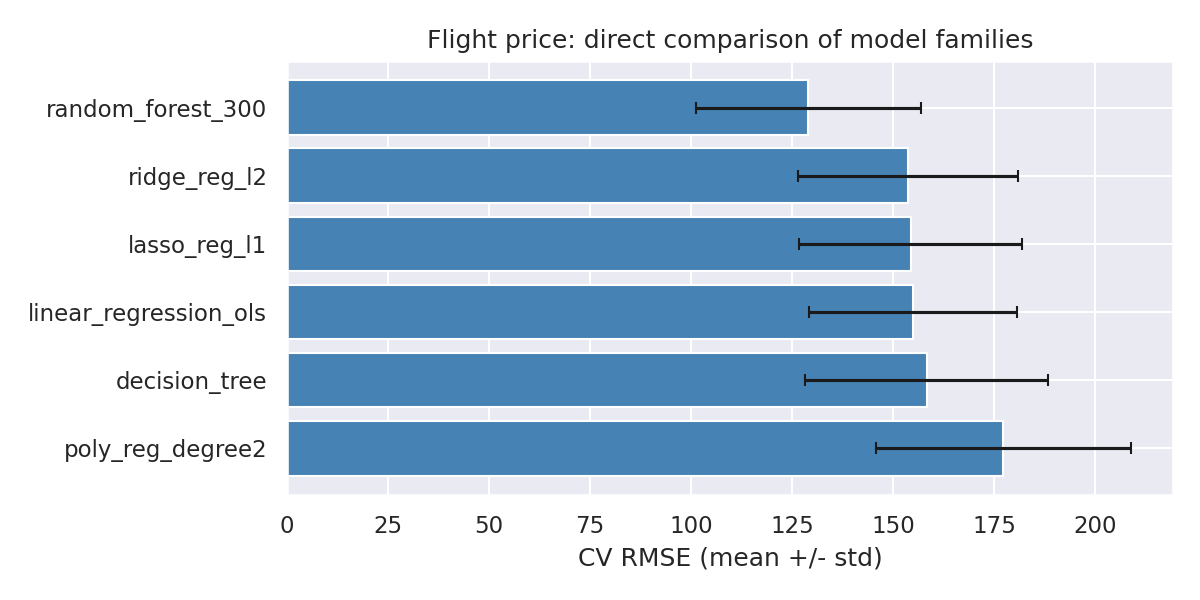
\includegraphics[width=0.72\linewidth]{flight_model_comparison.png}
\caption{Direct comparison of the model families (CV RMSE).}
\label{fig:flightcomp}
\end{figure}

\section{Hyper-parameter tuning}\label{sec:tuning}
\subsection{Polynomial regression: optimal degree}

Since the polynomial expansion is the natural way to give a linear model curvature, we tune its degree first. The degree controls how much curvature and interaction the model can represent: degree 1 is a straight line, degree 2 adds squares and pairwise products, and degree 3 adds triple products. We loop over degrees 1 to 3, fit OLS and Ridge ($\lambda=1$) on each expansion and plot the curves (Figure~\ref{fig:flightdegree}).

\begin{table}[H]
\centering
\small
\begin{tabular}{@{}lrr@{}}
\toprule
Polynomial degree & CV RMSE, L2 ($\lambda=1$) & CV RMSE, no penalty \\
\midrule
1 & 153.6 & 154.8 \\
2 & 136.7 & 177.3 \\
3 & 158.0 & 380.9 \\
\bottomrule
\end{tabular}
\caption{Polynomial regression: cross-validated RMSE by degree.}
\label{tab:flightdegree}
\end{table}

Degree 2 without a penalty is worse than degree 1 at 177.3 RMSE, and degree 3 goes up to 380.9 RMSE. With this much flexibility the model fits individual training rows, including noise and hence has high validation error. The same degree-2 expansion with an L2 penalty gives 136.7 RMSE, which is the best linear model we have seen so far. Hence we choose this for further experimentation with Ridge and Lasso regularization.

\begin{figure}[H]
\centering
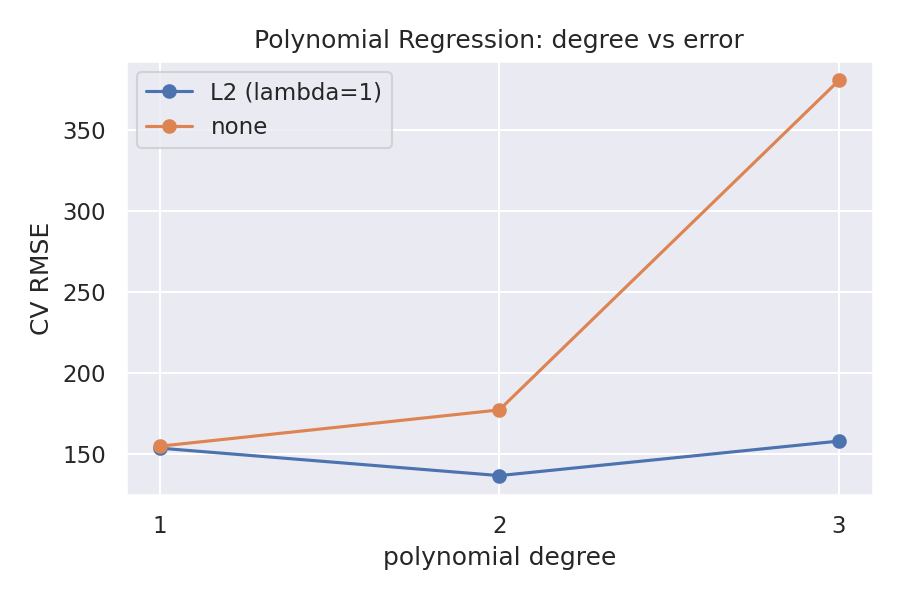
\includegraphics[width=0.56\linewidth]{flight_poly_degree.png}
\caption{Polynomial degree against Cross Validation (CV) error, with and without an L2 penalty.}
\label{fig:flightdegree}
\end{figure}

\subsection{Ridge and Lasso regularisation}

Ridge minimises the squared error plus $\lambda\lVert w\rVert_2^2$. A larger $\lambda$ shrinks the coefficients more. We iterate over $\lambda \in \{0.01,\dots,1000\}$ and plot the curve (Figure~\ref{fig:flightlambdas}, left). The curve is flat between $\lambda=1$ and 100 (152.9 to 154.6 RMSE), with the best value at $\lambda=10$ (152.9).

Lasso minimises the squared error plus $\lambda\lVert w\rVert_1$. For coefficient $w_j$ the optimality condition is
\[
  \frac{2}{n}\,\mathbf{x}_j^\top(\mathbf{y}-\mathbf{X}w) = \lambda\,s_j,
  \qquad s_j \in \partial|w_j|,
\]
so a coefficient is set to zero whenever $\bigl|\frac{2}{n}\mathbf{x}_j^\top(\mathbf{y}-\mathbf{X}w)\bigr| \le \lambda$. We iterate over $\lambda$ from $10^{-4}$ to 1, refit the best value and count the remaining features. Lasso has the best result at $\lambda=0.5$ with 154.1 RMSE, slightly behind Ridge, with 42 non-zero features out of 63 encoded features.

\begin{figure}[H]
\centering
\begin{subfigure}{0.49\linewidth}
  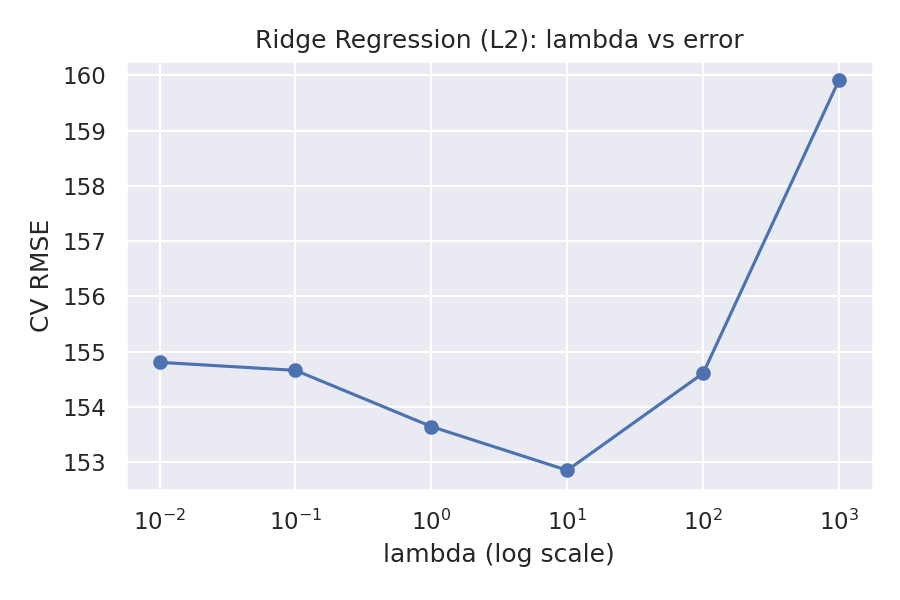
\includegraphics[width=\linewidth]{flight_ridge_lambda.png}
  \caption{Ridge}
\end{subfigure}
\hfill
\begin{subfigure}{0.49\linewidth}
  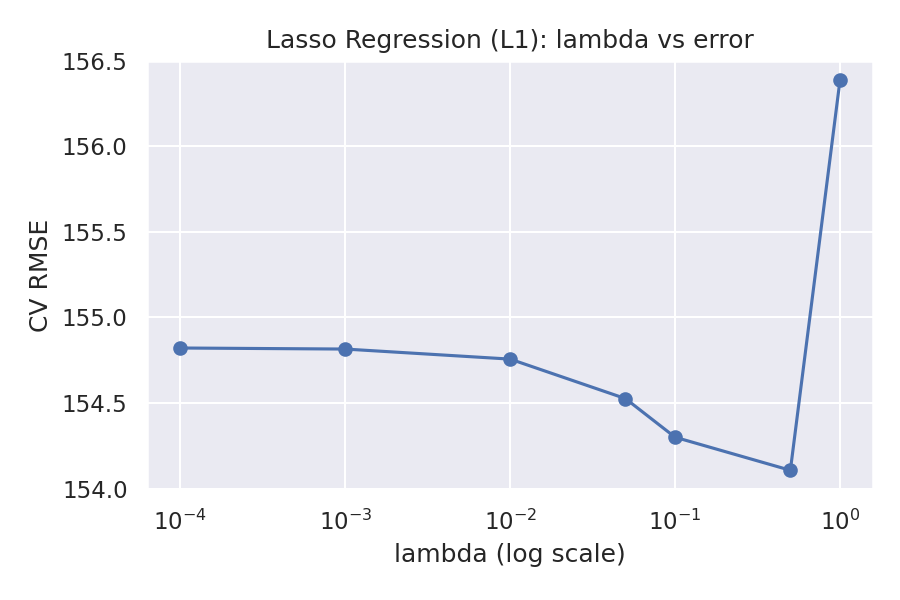
\includegraphics[width=\linewidth]{flight_lasso_lambda.png}
  \caption{Lasso}
\end{subfigure}
\caption{Regularisation curves.}
\label{fig:flightlambdas}
\end{figure}

\subsection{Decision tree: pre-pruning and post-pruning}

An unrestricted tree grows until its leaves are maximally pure. Hence to restrict overfitting, we carry out pre-pruning, for which we tune four limits together: maximum depth, minimum samples per leaf, minimum samples needed to split a node, and the maximum number of leaves. We observe best performance with depth 12 with a minimum leaf size of 5, having 128.8 RMSE.

For post-pruning we grow the tree fully and cut it back with the following cost-complexity criterion
\[
  R_\lambda(T) = R(T) + \lambda |T|,
\]
where $R(T)$ is the training error and $|T|$ the number of leaves, so $\lambda$ is the penalty per leaf. Pruning back to 66 leaves ($\lambda = 66.2$) gives about 148 RMSE, worse than the pre-pruned tree at 128.8, hence we keep the pre-pruned tree (Figure~\ref{fig:flightpruning}).

\begin{figure}[H]
\centering
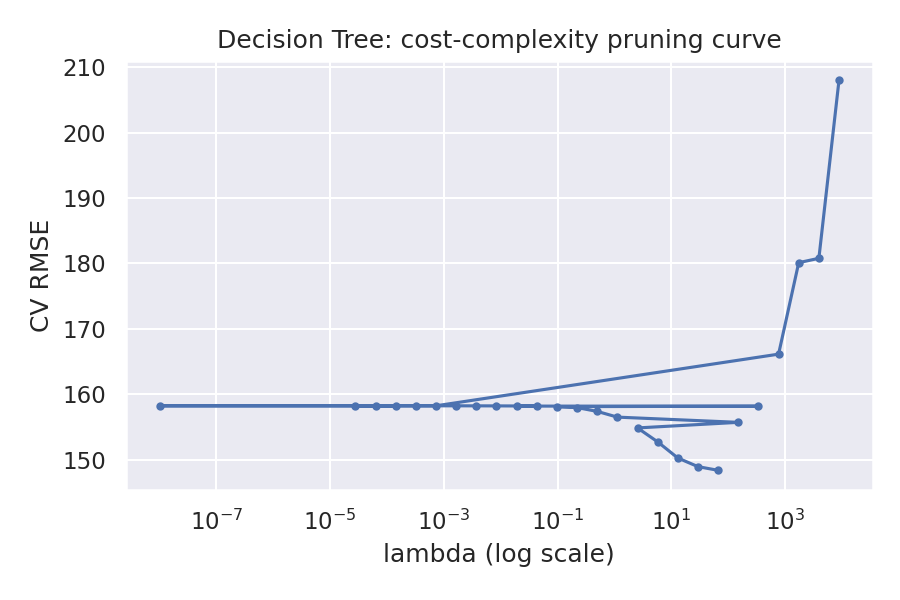
\includegraphics[width=0.56\linewidth]{flight_tree_pruning.png}
\caption{Cost-complexity pruning curve.}
\label{fig:flightpruning}
\end{figure}

\subsection{Random forest}

The random forest averages many decorrelated trees. We vary the number of trees and the minimum leaf size, keep the features per split at \texttt{"sqrt"}, and leave the depth unconstrained because the leaf size already limits the trees. Every configuration with leaf size 3 scores around 121.5 RMSE, while leaf size 1 has nearly 129. Doubling the number of trees from 200 to 400 changes the score by a fraction of an RMSE unit, so we keep the version with 400 trees and leaf size 3 (in favor of model complexity).

\section{Experiment: Regression on $\log(\text{price})$}

Since the target is heavily skewed (as we earlier observed), we test whether training on a transformed target helps the linear models. A handful of tickets cost more than USD 8,000 while the median is USD 234, so with squared error those rows will have an outsized weight.

We wrap the polynomial Ridge in a transformed-target regressor (\texttt{func=log1p}, \texttt{inverse\_func=\allowbreak expm1}), which fits the model on relative errors and converts the predictions back to dollars before scoring. Least-squares on the log scale is equivalent to least-squares on the log of a multiplicative error and is far less affected by the extreme values than OLS on the raw scale. We try this against degrees 1 and 2 with $\lambda \in \{0.1,1,10,100\}$ and re-evaluate the best performer according to the $R^2$ scores. \footnote{C. Tofallis, ``A better measure of relative prediction accuracy for model selection and model estimation'', \emph{Journal of the Operational Research Society}, 66(8):1352--1362, 2015, \S3.1 and \S3.3.}

The best configuration is degree 2 with $\lambda=10$, at about 125.0 RMSE and $R^2 = 0.6824$, against 136.7 for the degree-2 Ridge on the raw price. Even after this, the random forest (about 121.4 RMSE) stays ahead, so this regression model (log-price Ridge) is our strongest linear model as of yet.

\section{Experiment: Ensemble of Random Forest and Polynomial Regression with Ridge Regularization}

Since we have two very different models performing pretty well as of now, we try testing whether averaging them helps. Two combinations are tried with \texttt{VotingRegressor}: the random forest together with the log-price Ridge, and random forest + log-price Ridge + plain Ridge.

The first combination scores about 120.0 RMSE, slightly better than random forest alone at 121.4, while the second variation scores about 125.7. Since the gap is fairly low, in favour of lesser complexity, we keep the single random forest model as the best.

\section{Experiment: Testing the Random Forest with More Trees and More Features per Split}

In the earlier sections, we saw that the random forest with 400 trees and max\_features='sqrt' performed the best. Here we test the same model with more trees and with max\_features raised to 0.5 and 0.3, so each split can consider more columns. Along with this we add the count features and the duration ratio, and re-check the log-price Ridge on the new columns. 5-fold cross-validation is also carried out here like for the previous model evaluations.

\begin{table}[H]
\centering
\small
\setlength{\tabcolsep}{5pt}
\begin{tabular}{@{}>{\raggedright\arraybackslash}p{7.6cm}rrr@{}}
\toprule
Candidate & RMSE & MAE & $R^2$ \\
\midrule
Random forest (1000, 50\% features, leaf 3, extended, with id) & 117.10 & 42.59 & 0.7209 \\
Random forest (1000, 50\% features, leaf 3, extended) & 118.15 & 43.39 & 0.7160 \\
Random forest (800, 30\% features, leaf 2, extended) & 119.63 & 44.78 & 0.7090 \\
Random forest (1000, sqrt, leaf 3, extended) & 120.26 & 49.90 & 0.7058 \\
Random forest (400, sqrt, leaf 3, extended) & 120.33 & 49.91 & 0.7054 \\
Random forest (400, sqrt, leaf 3, base features) & 121.37 & 50.97 & 0.7003 \\
Log-price Ridge (deg 2, $\lambda=10$, extended) & 127.00 & 54.98 & 0.6718 \\
\bottomrule
\end{tabular}
\caption{Candidates in the second tuning round.}
\label{tab:retune}
\end{table}

With the variations described above, we could observe that raising max\_features to 0.5 with 1000 trees improves the score the most. The RMSE falls from 121.37 to 118.15 and the MAE from 51.0 to 43.4, so the model also tracks typical fares much better. The count features on their own give only a small improvement (121.37 to 120.33), and doubling the trees without changing anything else changes nothing measurable (120.26).

We can conclude that the gains have saturated at this point. Since the log-price Ridge does worse once the count columns are added, the random forest remains the stronger choice against the linear family. The row "id" is not used as a feature anywhere else, but it has some correlation with the price, that is, a slow decline across the dataset. Adding it as an extra column gives another small improvement. This achieves 117.1 RMSE and $R^2$ 0.721, and its public leaderboard score on Kaggle is 0.76352.

\subsection{An 80/20 test of the the above models}

We test the above modified random forest on the 20\% of the training rows kept aside, and also refit it on a much smaller subset to see how much it depends on the training volume:

\begin{table}[H]
\centering
\small
\setlength{\tabcolsep}{6pt}
\begin{tabular}{@{}>{\raggedright\arraybackslash}p{6.4cm}lrrr@{}}
\toprule
Model & Training rows & RMSE & MAE & $R^2$ \\
\midrule
Random forest with id (1000, 50\% features, leaf 3) & 80\% & 91.79 & 41.33 & 0.7902 \\
Random forest with id (1000, 50\% features, leaf 3) & 20\% & 105.47 & 54.75 & 0.7230 \\
Random forest (1000, 50\% features, leaf 3) & 80\% & 93.53 & 42.32 & 0.7822 \\
Random forest (1000, 50\% features, leaf 3) & 20\% & 104.42 & 54.26 & 0.7285 \\
Log-price Ridge (deg 2, $\lambda=10$) & 80\% & 110.00 & 53.72 & 0.6987 \\
Log-price Ridge (deg 2, $\lambda=10$) & 20\% & 109.00 & 58.44 & 0.7042 \\
\bottomrule
\end{tabular}
\caption{Scores on the unseen 20\% of the training data.}
\label{tab:flightholdout}
\end{table}

\begin{figure}[H]
\centering
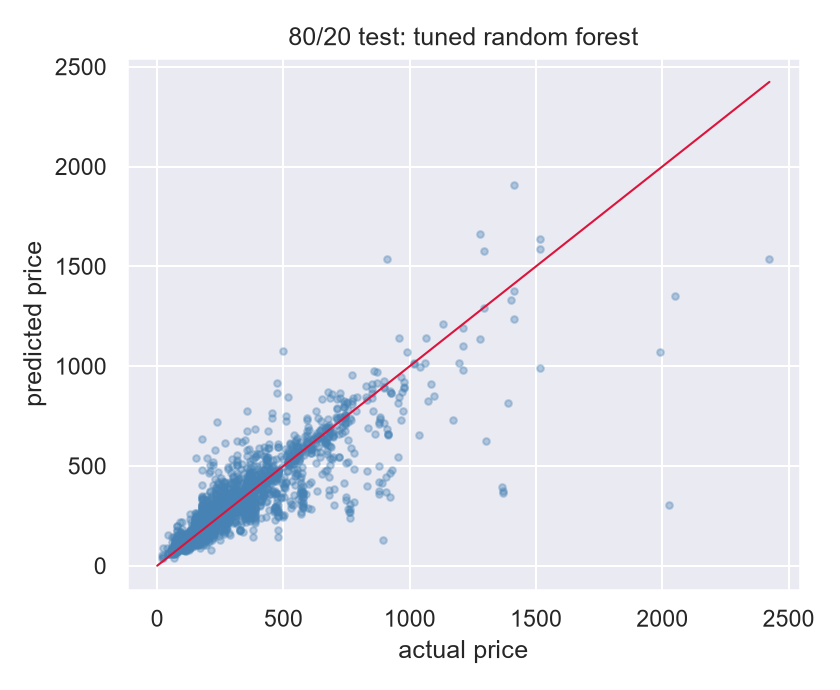
\includegraphics[width=0.62\linewidth]{flight_80_20_test.png}
\caption{The tuned random forest on the unseen 20\% of the training data.}
\label{fig:flightholdout}
\end{figure}

When trained on 80\% of the rows the random forest reaches $R^2$ 0.782 on the unseen 20\%, against 0.729 when trained on only 20\% of the rows, so it still benefits from data volume. Adding the id column improves the score again, to $R^2$ 0.790.

\section{Experiment: Ensemble of HistGradientBoosting + Random Forest + ExtraTrees}

In parallel with the tuning above, we also tested a combination / blended ensemble with another set of 21 engineered features (eight numeric columns, eight label-encoded categoricals and five frequency counts over composite keys). Three tree models were trained on it: histogram-based gradient boosting (500 iterations, 63 leaves), a random forest (200 trees, half the features per split) and an extra-trees model (300 trees, 70\% of the features per split). Each was scored with the same 5-fold cross-validation.

\begin{table}[H]
\centering
\small
\setlength{\tabcolsep}{6pt}
\begin{tabular}{@{}>{\raggedright\arraybackslash}p{6.8cm}rrr@{}}
\toprule
Model & CV RMSE & CV $R^2$ & Public LB \\
\midrule
Histogram gradient boosting (500 iterations) & 122.32 & 0.6963 & \\
Random forest (200 trees, 50\% features) & 122.85 & 0.6937 & \\
Extra trees (300 trees, 70\% features) & 124.05 & 0.6876 & \\
Blend (weights 0.54 / 0.30 / 0.17) & 120.82 & 0.7037 & 0.76298 \\
Blend, cleaned rows and id column & 119.38 & 0.7105 & 0.76320 \\
\bottomrule
\end{tabular}
\caption{The blended ensemble on the compact feature frame.}
\label{tab:blend}
\end{table}

We could observe that this combination of models improved on each of its members (120.8 against 122.3 RMSE), producing our best public leaderboard score on Kaggle, 0.78058.

\section{Model diagnostics}
\subsection{Predicted vs actual (out-of-fold)}

We collect out-of-fold predictions for the random forest and the log-price Ridge and plot them against actual prices (Figure~\ref{fig:flightpred}). In both panels most points stay close to the diagonal for ordinary fares (up to roughly USD 1,500), and both models under-predict the rare expensive tickets. The random forest predictions rarely exceed USD 2,000 even when the actual price is far higher, which is expected, since trees average leaf values, and expensive tickets are too rare to form their own leaves.

\begin{figure}[H]
\centering
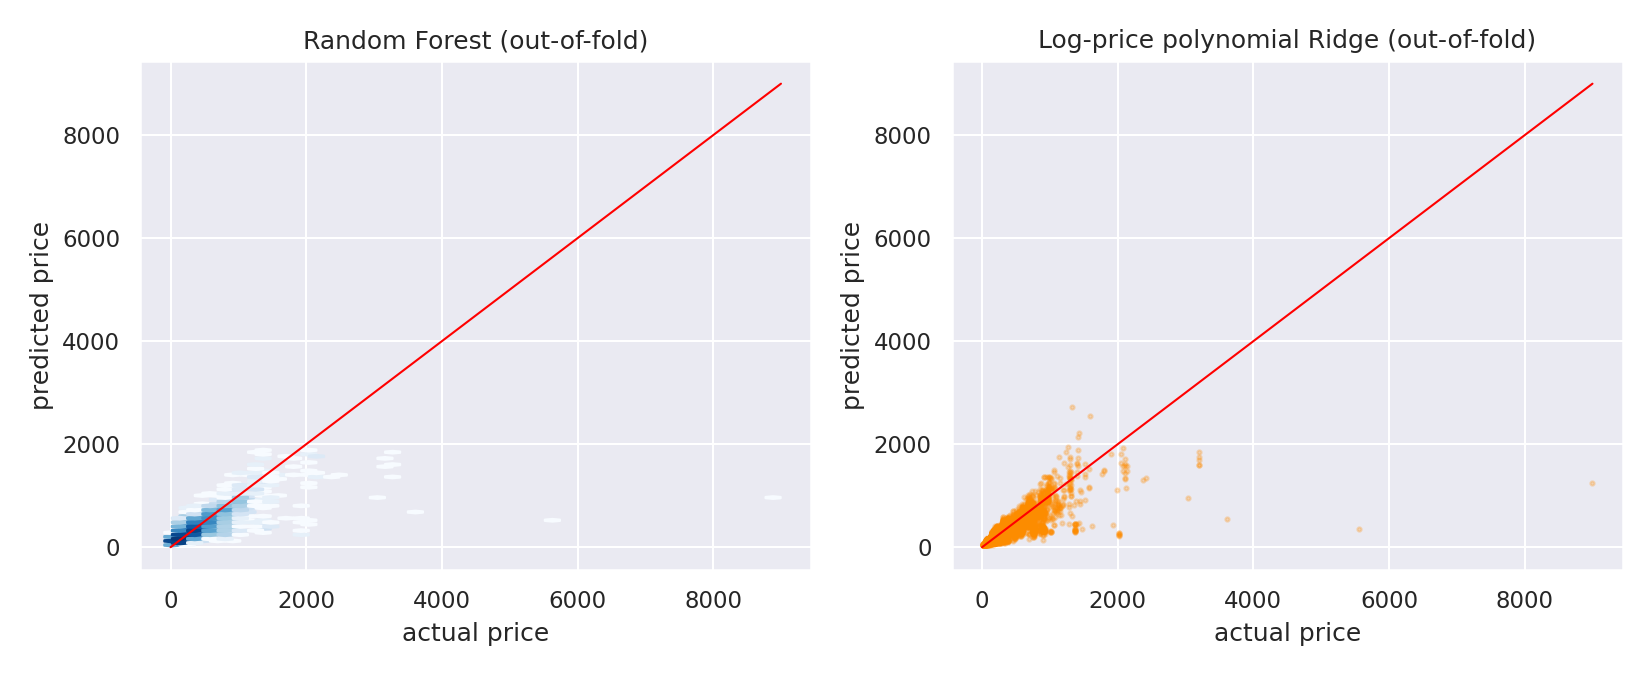
\includegraphics[width=\linewidth]{flight_pred_vs_actual.png}
\caption{Out-of-fold predicted vs actual price.}
\label{fig:flightpred}
\end{figure}

\subsection{Residual analysis (random forest)}

We compute the residuals $e_i = y_i - \hat{y}_i$ for the random forest and plot their histogram and their values against the predictions (Figure~\ref{fig:flightres}). The histogram is centred close to zero (mean $-0.18$) with a small number of large positive residuals, which occur only where the model predicted a high price.

\begin{figure}[H]
\centering
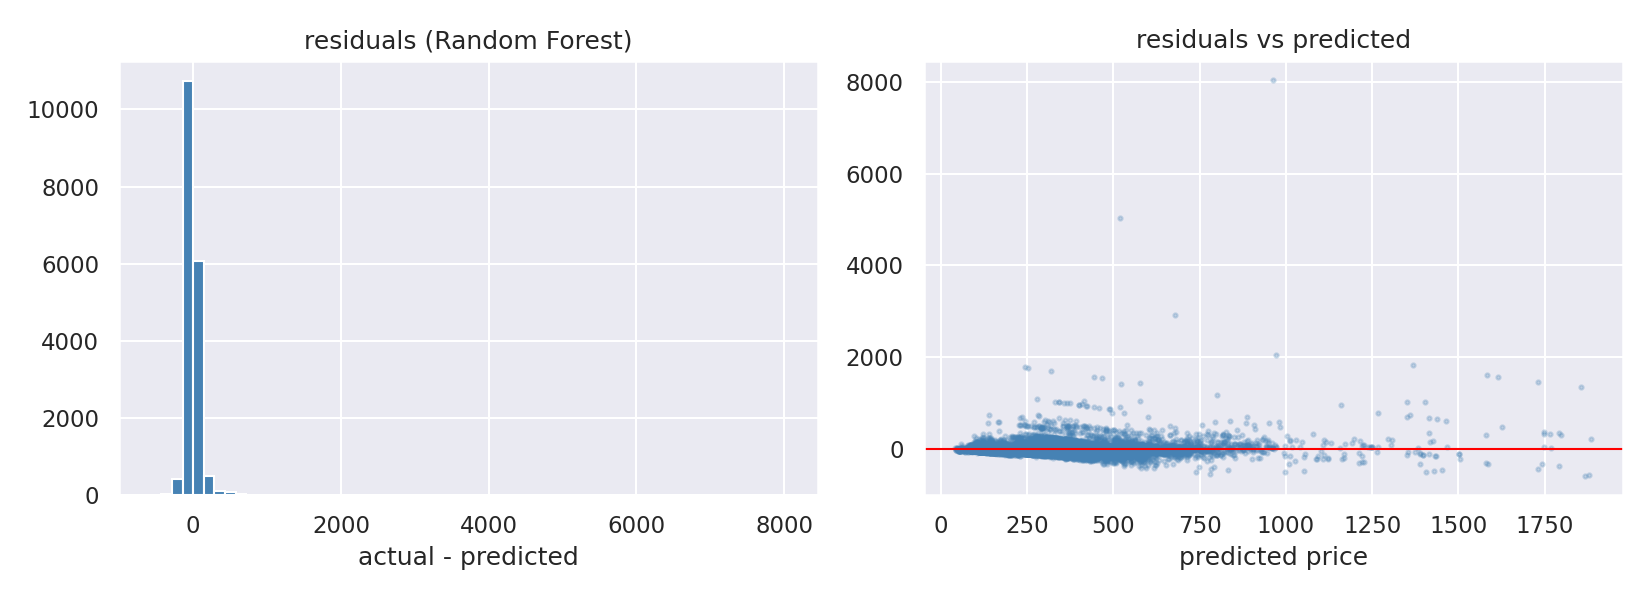
\includegraphics[width=\linewidth]{flight_residuals.png}
\caption{Random forest residuals: histogram and residuals against predictions.}
\label{fig:flightres}
\end{figure}

\subsection{Feature importance (random forest)}

Finally, we refit the random forest on all training rows and draw the 15 largest impurity importances (Figure~\ref{fig:flightimp}). The booking window, the flight length and the seating class affect the price the most, and the engineered columns are also seen to be of actual use: \texttt{flight\_number} (0.05), \texttt{stops\_ordinal} (0.05), the stop indicators and the Sacramento-San Jose route (0.036) all appear before the remaining categories.

\begin{figure}[H]
\centering
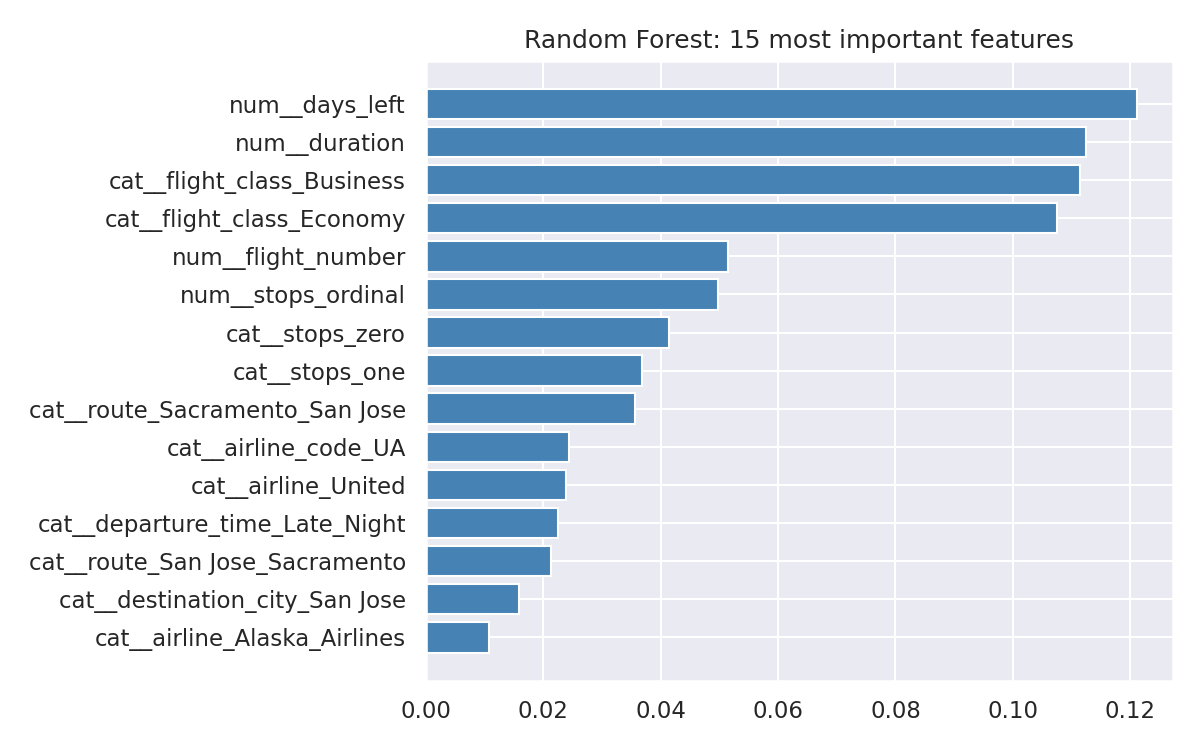
\includegraphics[width=0.62\linewidth]{flight_rf_importance.png}
\caption{Random forest feature importances.}
\label{fig:flightimp}
\end{figure}

\section{Cross-validation of shortlisted models}

Since a single 5-fold estimate can shift with the fold split, we re-evaluate the three finalists with 5 folds repeated 3 times (15 scores each): the random forest (121.30 $\pm$ 32.18), the pre-pruned tree (130.01 $\pm$ 31.75) and the log-price Ridge (124.86 $\pm$ 30.69). 


\section{Metrics comparison}

\begin{table}[H]
\centering
\small
\setlength{\tabcolsep}{5pt}
\begin{tabular}{@{}>{\raggedright\arraybackslash}p{6.2cm}rrr@{}}
\toprule
Model & RMSE & MAE & $R^2$ \\
\midrule
Random forest (400, sqrt, leaf 3) & 121.37 & 50.97 & 0.7003 \\
Log-price polynomial Ridge (deg 2, $\lambda=10$) & 124.96 & 55.30 & 0.6824 \\
Decision tree (depth 12, leaf 5) & 128.82 & 49.31 & 0.6624 \\
Polynomial Ridge (deg 2, $\lambda=1$) & 136.67 & 60.86 & 0.6120 \\
Decision tree, cost-complexity pruned & 148.39 & 65.21 & 0.5428 \\
Ridge (L2, $\lambda=10$) & 152.85 & 80.32 & 0.5244 \\
Lasso (L1, $\lambda=0.5$) & 154.11 & 80.33 & 0.5168 \\
Linear regression (OLS) & 154.82 & 80.42 & 0.5107 \\
Polynomial regression (deg 2, no penalty) & 177.25 & 62.56 & 0.2742 \\
\bottomrule
\end{tabular}
\caption{Flight price: full metrics comparison.}
\end{table}

From the table, the random forest is best on RMSE and $R^2$ (121.4, 0.70) and second on MAE (51.0), behind the pre-pruned tree (49.3); the log-price polynomial Ridge is the best linear-family model (125.0, 0.68), while the plain polynomial and unregularised variants are the weakest.

We can observe via the MAE values that the tree-based models track typical fares well but end up having decreased performance due to for larger errors on expensive tickets. 

\section{Submission CSV Creation and Best Model Choice}

We fit every model on all training rows and write one CSV per model.

\begin{table}[H]
\centering
\caption{Best model and its submission.}
\label{tab:final}
\small
\begin{tabular}{@{}>{\raggedright\arraybackslash}p{4.6cm}cc>{\raggedright\arraybackslash}p{3.4cm}@{}}
\toprule
Final model & CV score & Public LB & Submission file \\
\midrule
Random forest, 1000 trees, 50\% features, leaf 3, with id & $R^2$ 0.7209 & 0.76352 & \texttt{submission.csv} \\
\bottomrule
\end{tabular}
\end{table}

The public scores of the various models we tested were: log-price Ridge 0.70155, pre-pruned tree 0.69389, pruned tree 0.64657, polynomial regression 0.63352, Ridge 0.55503, Lasso 0.54922, OLS 0.53131, and the forest plus Ridge ensemble 0.74533; the tuned forest and its variant having the id column were 0.75904 and 0.76352 and we achieved the best public score with the ensemble of HistGradientBoosting + Random Forest + ExtraTrees (best model).

\section{Conclusion}

\begin{itemize}
  \item The target is heavily skewed, so the squared error is sensitive to the rare expensive tickets and the cross-validation scores are spread widely.
  \item Cleaning out data errors (like the 25 flights priced at zero) and building custom features helped increase performance, as seen in the feature importance of the airline code, flight number, exact route and number of stops for the random forest models.
  \item Our basic degree-3 polynomial completely overfit the data; decreasing to degree 2 and adding a small L2 penalty (Ridge) gave us our best linear model at 136.7 RMSE. With the Lasso penalty as well, we could match that performance (and it ignored about a third of our features, keeping the model less complex).
  \item When tuning the decision trees, setting up limits before training (pre-pruning) worked much better than trimming the tree after it grew (128.8 against 148 RMSE).
  \item Transforming our target to predict the log of the price increased the performance of the linear models manifold. We tried averaging that log-price Ridge model with the random forest, which nudged the overall RMSE down to 120.0, but it was only a marginal gain for increased complexity, so we did not go forward with that.
  \item We also tried the random forest with more trees and max\_features at 0.5 together with the new count features. That brought the RMSE down to 118.2 and the MAE to 43. A blended ensemble of boosting and tree models scored 0.78058, hence becoming our best model.
\end{itemize}

\end{document}
